\documentclass{IEEEcsmag}

\usepackage[colorlinks,urlcolor=blue,linkcolor=blue,citecolor=blue]{hyperref}

\usepackage{tabularx}
\usepackage{upmath}
\usepackage{amssymb}
\usepackage{amsmath}
\usepackage{array}
\usepackage{arydshln}
\usepackage{listings, multicol}
\usepackage{filecontents}
\usepackage{parcolumns}


\newcolumntype{P}[1]{>{\centering\arraybackslash}p{#1}}

\jvol{XX}
\jnum{XX}
\paper{8}
\jmonth{May/June}
\jname{Computing in Science and Engineering}
\pubyear{2021}
\newtheorem{theorem}{Theorem}
\newtheorem{lemma}{Lemma}

\setcounter{secnumdepth}{0}

\lstset{language=Python, basicstyle=\ttfamily\footnotesize}

\begin{filecontents*}{loop_fusion.py}
import numba
import numpy as np

# optionally the decorator can take
# the option nopython=True, which
# disallows Numba from running in
# object mode
@numba.jit
def loop_fusion(a):
    """
    An example of loop fusion, an
    optimization that Numba is able
    to perform on a user's behalf.
    When it recognizes that they are
    operating similarly on a single
    data structure
    """
    for i in range(10):
        a[i] += 1

    for i in range(10):
        a[i] *= 5

    return a
\end{filecontents*}

\begin{filecontents*}{nested_function.py}
import numpy as np
import numba
import numba.core
import numba.typed


# Dictionary instance created at runtime
results = numba.typed.Dict.empty(
    key_type=numba.core.types.unicode_type,
    value_type=numba.core.types.float64[:]
)

@numba.njit
def nested(input, results):
    # This function expects a
    # typed dictionary as an
    # argument to store results

    def step1(a):
        # first step of algorithm
        # store results in dictionary
        ...

    def step2(a):
        # second step of algorithm
        # store results in dictionary
        ...

    return results

\end{filecontents*}

\begin{filecontents*}{parallel_multithreading.py}
import numba
import numpy as np

@numba.njit(cache=True, parallel=True)
def multithreading(a):

	for i in numba.prange(10):
		a[i] *= 10

\end{filecontents*}


\begin{document}

\sptitle{Department: Head}
\editor{Editor: Name, xxxx@email}

\title{PyExaFMM, an exercise in designing high-performance software with Python and Numba}

\author{S. Kailasa}
\affil{Department of Mathematics, University College London}

\author{T. Wang}
\affil{Department of Mechanical and Aerospace Engineering, The George Washington University}

\author{\text{L}. A. Barba}
\affil{Department of Mechanical and Aerospace Engineering, The George Washington University}

\author{T. Betcke}
\affil{Department of Mathematics, University College London}

\markboth{Department Head}{Paper title}

\begin{abstract}
    Numba is a game changing compiler for high performance computing with Python. The machine code it produces runs outside of the single-threaded Python interpreter, and can therefore fully utilize the resources of modern CPUs. This means support for parallel multithreading and auto vectorization if available, just like in a compiled language such as C++ or Fortran. Here we document our attempt to use Numba to develop a fully multithreaded implementation of the Fast Multipole Method, an algorithm which relies on a non-linear data structure and contains a significant amount of data organization that would ordinarily be run through the Python interpreter. We explain how Numba significantly influences the design and structure of software, as well as its major pitfalls when designing complex implementations. We find that Numba doesn't live up to its promise due to overhead from the unavoidable interaction between the Python interpreter and Numba compiled code, and that our software remains an order of magnitude slower than ExaFMM-T, the leading C++ implementation of the same algorithm.
\end{abstract}

\maketitle
\chapterinitial{Python}\footnote{We use `Python' to refer to CPython, the popular C language implementation of Python, which is dominant in computational science.}, is designed for memory safety and developer productivity, not speed. Its main selling point being that it allows Computational Scientists to spend more time exploring the science, and less time being confused by strange software quirks, infuriating memory errors, and the nightmare of incompatible dependencies, all of which conspire to drain productivity when working with lower level languages.

The catch is that code is run through an interpreter and restricted to run on a single thread via a software construction called the Global Interpreter Lock [GIL]. However, libraries for high performance computational science have traditionally bypassed the issue of the GIL by using Python's C interface to call extensions built in C or other compiled languages which can be multithreaded and compiled to target special hardware features. Popular examples of this approach include Numpy and SciPy, which together have helped propel Python's popularity in computational science by providing high performance data structures for numerical data as well as interfaces for fast compiled implementations of algorithms for numerical linear algebra, and mathematical solvers for problems from differential equations to statistics and machine learning.

As the actual number-crunching itself happens outside of the interpreter, the GIL only becomes a bottleneck to performance if a program must repeatedly pass control between the interpreter and non-Python code. This is most often an issue when an optimized compiled language implementation of your desired algorithm doesn't exist in the Python Open Source, or if it requires a lot of data organization to form the input for an optimized Numpy or SciPy code, which must unavoidably take place within the interpreter. Previously, an unlucky developer would have been forced to write a compiled implementation to tackle these issues themselves and connect it to their Python package, relegating Python's role to an interface. More problematically, not all Computational Scientists have the necessary software skills or research interest in developing and maintaining complex codebases that couple multiple languages.

This is the context in which Numba was introduced \cite{Lam2015}. It is a compiler that specifically targets and optimizes Python code written with Numpy's ndarray data structure. Its power comes from the ability to generate multithreaded architecture optimized compiled code while \textit{only writing Python}. The promise of Numba is the ability to develop applications with speed that can rival C++ or Fortran, while retaining the simplicity and productivity of working in Python. We put this promise to the test by developing PyExaFMM\footnote{https://github.com/exafmm/pyexafmm}, an implementation of the Kernel-Independent Particle Fast Multipole Method [FMM] \cite{Ying2004,Greengard1987}, in three dimensions. Efficient implementations of this algorithm are complicated by a recursively defined tree data structure and a series of operations which each require significant data organization and careful memory allocation. These features made PyExaFMM an excellent test case to see whether Numba could free us as Computational Scientists from the complexities of compiled languages.

We begin with an overview of Numba, focussing on when and where its use is appropriate and its major pitfalls. After introducing the necessary concepts of the FMM such as its data structure and the computations involved, we provide an overview of how we designed our software's data structures, algorithm implementations, and application programming interface [API] to optimally use Numba. We conclude benchmarks demonstrating the impact of Numba on vanilla Python implementations of the FMM's operators, the cost of passing between the Python interpreter and Numba compiled code, and performance in terms of memory and runtime in comparison to ExaFMM-T \cite{Wang2021}, the leading C++ implementation of the same algorithm. We note that a strict like-for-like comparison between the two implementations isn't possible. The softwares take different approaches to the implementation of some of their operations and data structures. However, as the differences in the design of PyExaFMM are heavily influenced by Numba and Python, it remains useful as an illustration of what can be achieved with Python in comparison to a compiled language to solve the same problem.

\section{NUMBA}

Numba\footnote{We use the latest stable release of Numba, 0.53.1 throughout this study.} is a compiler for Python, and was initialy developed to optimize a subset of the language that manipulates the $n$-dimensional array, or `ndarray', data structure from Numpy. Unlike a Python list, where elements can be of any type and are linked by a chain of pointers, ndarrays are homogeneously typed and stored contiguously in memory. This means that adjacent elements are stored in adjacent memory locations. When loading data from a given memory location, modern CPUs cache data located at adjacent locations, therefore algorithms which iterate sequentially over arrays benefit from lower memory loading latencies as the CPU's cache is likely to contain the next element being operated on. This is known as \textit{locality of reference}. This is in contrast to Python lists, where subsequent elements need not be stored in adjacent memory locations and are found by following trails of pointers, this phenomena is known as \textit{indirection}, which doesn't take advantage of CPU caching behavior at all. As ndarrays have fields for data dimensionality, type, and layout, Numba can use this to generate machine code without any indirection. instead it can directly reference the memory locations being referred to by the Python code at runtime. This allows Numba to index into ndarrays with performance that can match compiled languages.

Numba is built with LLVM \cite{Lattner2004}, a framework for building custom compilers, that provides an API to generate machine code for different hardware architectures such as CPUs and GPUs. LLVM is also able to analyze the code it's compiling for hardware level optimizations, such as auto vectorization, and apply them automatically if they are available on the target hardware.

From a programmer perspective, using Numba naively doesn't involve a significant rewrite of code. Functions in the Python source code are marked for compilation with a special decorator (see listings (\ref{code:loop_fusion}) and (\ref{code:parallel_multithreading}) for example syntax). if a marked function is called at runtime from the Python interpreter, program execution is handed to Numba's runtime, which then compiles the function on the fly with a type signature matching the types of the input arguments. This is the origin of the term `just in time' [JIT] to describe such compilers.

Figure (\ref{fig:numba}) illustrates the program execution path when a Numba decorated function is called from the Python interpreter. We see that Numba doesn't replace the Python interpreter. Instead, a special Numba runtime program interacts with the Python interpreter dynamically and the control of program execution is passed back and forth between Numba and Python. There is an inherent cost to this interaction which from having to `unbox' Python objects into types compatible with the compiled machine code, and `box' the outputs of the compiled functions back into Python compatible objects. This process doesn't involve re-allocating memory, however pointers to memory locations have to be converted and placed in a type compatible with either Numba's compiled code or Python. The cost of this can be seen in Table ([REFERENCE TO BOX BENCHMARK TABLE]), where we illustrate the cost of boxing and unboxing functions of with increasing numbers of array arguments. Table ([REFERENCE BOX BENCHMARK FOR DIFFERENT TYPES]) illustrates the cost of boxing different Python types into Numba compatible types. Software written with Numba has to account for this cost, and minimize the interactions between the Python interpreter and Numba compiled code.

\lstinputlisting[float=t, caption={An example of using Numba in a Python function operating on ndarrays.}\label{code:loop_fusion}]{loop_fusion.py}

\section{PITFALLS OF NUMBA}

Since it was first released, Numba has been extended to compile most functionality from the Numpy library seamlessly, as well as a wide variety of well loved Python language data structures, functions and standard library modules \footnote{A full list of supported features for the current release can be found at: https://numba.pydata.org/numba\-doc/dev/reference/pysupported.html}. However, If Numba isn't able to find a suitable Numba type for each Python type in a decorated function, or it sees a Python feature it doesn't yet support, it runs in `object' mode, and handles all values as generic Python objects using Python's underlying C implementation to handle operations on these objects. Crucially Numba does this without reporting it to the user, with object mode often no faster than ordinary vanilla Python code. This puts the burden on the programmer to understand when and where Numba might work. Furthermore, to achieve performance, a programmer must be careful to limit the surface of interaction between Python code and Numba code. Therefore, in practice Numba behaves like a framework rather than just a compiler, as it influences the way in which you write Python.

Additionally, though a large number of Python features are supported, not everything is supported in a way a Python programmer would expect which can have impacts on program design. An example this situation arises when using Python dictionaries, which are partially supported by Numba. As they are untyped, and can have any Python objects as members, they don't neatly fit into a Numba compatible type. Programmers can declare a Numba compatible `typed dictionary', where the keys and values are constrained to Numba compatible types, and pass it to a Numba decorated function at low cost. However, using a Numba dictionary from the Python interpreter is always slower than an ordinary Python dictionary due to the (un)boxing cost when getting and setting any item. A natural use case for a dictionary is as a place to store results during an algorithm. To avoid the (un)boxing cost in algorithms that involve multiple steps that operate on shared data, programmers are forced write a nested functions as in listing (\ref{code:nested_function}) that are called as minimally as possible. These nested functions have the tendency to grow long in highly-performant Numba code, in order to keep the interaction surface between Numba and Python small. Therefore when pursuing performance with Numba, code can end up looking quite un-Pythonic, with few user created objects, performance critical sections written in terms of loops over simple array based data structures reminiscent of C, and many long nested functions which are uncommonly used in standard Python and are more difficult to unit test.

Though Numba is advertised as an easy way of injecting performance into your program via a simple decorator, achieving performance in practice may require a programmer to be familiar with the internals of its implementation (fig. \ref{fig:numba}), and potentially have to radically change the design of their algorithms and data structures to avoid back and forth between the Numba runtime and the Python interpreter. A significant proportion of Numba's intended target audience who are not software specialists may find it easier to stick with their C or Fortran implementations where performance is generally guaranteed regardless of implementation details.

\begin{figure*}
    \centerline{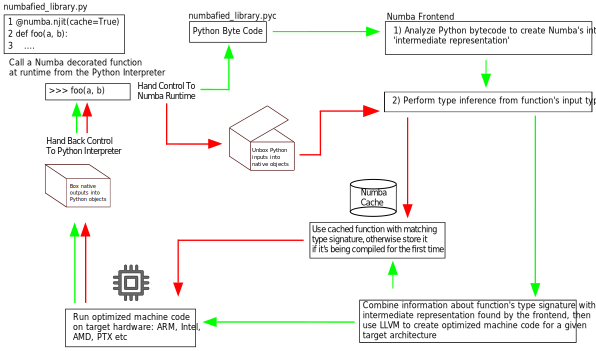
\includegraphics {figures/numba.pdf}}
    \caption{Simplified execution path when calling a Numba compiled function from the Python interpreter. The green path is only taken if the function hasn't been called before. The red path is taken if a compiled version with the correct type signature already exists in the Numba cache.}
    \label{fig:numba}
\end{figure*}



\lstinputlisting[float=t, caption={An example of using typed dictionaries in Numba.}\label{code:nested_function}]{nested_function.py}

\section{THE FAST MULTIPOLE METHOD}

The particle FMM is an approximation algorithm for $N$-body problems in which $N$ source particles interact with $M$ target particles \cite{Greengard1987}. Without loss of generality we can consider the sources and targets to correspond to the same set of particles. An example of this is the calculation of electrostatic potentials from a set of charged particles, and we use this as our reference problem to test the performance of our software. Consider a three-dimensional domain, with a set of $N$ charged particles at positions $x_i$. The potential, $\phi_j$, at a given particle at $x_j$ due to all other particles, excluding self interaction, can be written as.

\begin{equation}
    \phi_j = \sum_{i=1, i \neq j}^{N} \frac{q_i}{| x_i-x_j |}
    \label{eq:laplace_kernel}
\end{equation}

where $\frac{1}{| x_i-x_j|}$ is called the kernel, or the Green's function, and $q_i$ is the charge at $x_i$. The naive computation over all particles is $O(N^2)$, however the FMM compresses groups of interactions far away from a given particle to reduce the overall complexity to just $O(N)$, with a well described error bound for a chosen level of discretization. Problems with this structure appear frequently in science and engineering and are made tractable using the FMM, as a result it's been described as one of the ten most important algorithms of the twentieth century \cite{Cipra2000}. The algorithm relies on a hierarchical octree data structure to discretize the problem domain in three dimensions (see fig. 1 in \cite{Sundar2007}) and consists of eight operators: P2M, P2L, M2M, M2L, L2L, L2P, M2P and P2P applied during two consecutive traversals of the octree (bottom-up and then top-down). We defer to the FMM literature for a more detailed discussion on the mathematical significance and formulation of these operators \cite{Greengard1987}. The Kernel Independent FMM \cite{Ying2004}, implemented by PyExaFMM and ExaFMM-t, is a re-formulation of the FMM with a structure that favours parallelization. Indeed all of the operators can be decomposed into matrix-vector products, which fit well with Numba.

In formulating a parallelization strategy, the important quantities to understand are the computations involved and the whether there is any data being shared.

P2M

M2M

L2L

M2L

P2P (L2P, M2P, S2L)


% The depth of the octree is defined by a user provided value for $n_{crit}$, defining the maximum number of particles within a leaf node and hence defined by the distribution of particles. An operator is read as 'X to Y', where `P' stands for particle(s),`M' for \textit{multipole expansion} and `L' for \textit{local expansion}.

% These expansions are ways of describing the charge contained within subregions of the octree, and can be tuned to a given accuracy, described by a parameter called the expansion order, or $p$. A multipole expansion represents the aggregation of charge located with a given node of the octree, where the expansion center is set to coincide with the box center. A multipole expansion can be translated into a local expansion centered on another node, inside of which it is valid. This is nothing other than the M2L operator, therefore the operators can be seen to be translations between expansion representations. Similarly, the expansion centers of of local or multipole expansions can be shifted, which are the L2L and M2M operators respectively. The P2M/P2L operators forms a multipole/local expansion for a set of particles within a node. The M2P, L2P and P2P refer to directly evaluating the interaction in $O(N^2)$ between multipole/local expansion equivalent charges, or a set of source particles, at a set of target particles, respectively. % Multipole expansions are found by enclosing a node with an `equivalent surface' discretized with $n_e$ quadrature points, at each of which is placed an `equivalent charge'. A `check surface' discretized with $n_c$ quadrature points, is then used to enclose both the equivalent surface and the node, and a potential is calculated at the check surface using (\ref{eq:laplace_kernel}) directly with either the particles with the node (for P2M) or the equivalent charges of child nodes contained within the node (for M2M) as the source particles. Finally, a least-squares fit is used to match this calculated potential to that generated by the equivalent charges. Similar logic is used to calculate the M2L and L2L operators, with modified check and equivalent surfaces (see fig. 5 \cite{Ying2004}). The L2P, M2P, S2L and P2P operators all involve using (\ref{eq:laplace_kernel}) for direct evaluations, rather than a least-squares fit.


\section{MULTITHREADING IN NUMBA}

Numba implements threading in a platform agnostic way,  giving users the choice between OpenMP or IntelTBB backends. We choose the OpenMP backend, as the size of the tasks performed by FMM operators are approximately uniform, whereas TBB implements scheduling optimizations more suited to unbalanced workloads.

The P2M operator is only applied over the octree's leaves. The input data are the charges contained within each leaf, and their relevant surfaces, the operator outputting the multipole expansion. The calculation for the check potentials is $O(n_{crit} \cdot n_c)$ followed by $O(n_e \cdot n_c)$ for the multipole expansions for each leaf. This operator favours a parallelization over leaves as the calculations are independent.

The M2M operator finds the contribution to the multipole expansion of a given node due to the multipole expansions of all of its eight children. The input

when applied at a given octree level, $l$, its complexity is $O(8^l \cdot n_e \cdot n_c)$.
data required
complexity
parallelization strategy

L2L. serial - interaction
data required
complexity
parallelization strategy

M2L
data required
complexity
parallelization strategy

S2L
data required
complexity
parallelization strategy

M2P, S2P, S2L, P2P
Contextualize the computations required of each kernel. i.e. P2P is raw multithreading performance.
data required
complexity
parallelization strategy

- Multithreading api in numba, and make analogies with openmp where they exist. Link to recent efforts to implement an OpenMP interface within Numba?

- Thread oversubscription issues and their origin and how to avoid this in Numba. Comment on the quality of this solution - the py multithreading papers from intel group have good information and experiments regarding this.

- how kernels are multithreaded bearing in mind issues raise in Numba section, and data oriented design section.

- Optimal design of multithreading approach relies on the actual constraints of the kernel in question, will need to get into specifics here of how each kernel was approached.

- metric for portion of code that is run on single vs multiple threads, can actually time this at least roughly.

M2M
- serial. cannot parallelize over leaves, there are parallel writes to parent multipole expansion from siblings. Parallelizing over sibling leaves is hard due to linear representation of tree - have to perform expensive neighbours searches to find siblings to perform group by. equivalent charge = $O(8^l \cdot n_e \cdot n_c)$ at a given level $l$.

\lstinputlisting[float=t, caption={An example of parallel multithreading.}\label{code:parallel_multithreading}]{parallel_multithreading.py}

\section{DATA ORIENTED DESIGN}

- tree design
    - things this makes hard - neighbor searches.
    - things it makes easy - locality of reference, easy interoperability with numba
- API designed
    - Minimize the impact of running code in the interpreter.
- Software design diagram

% Larger figure
\begin{figure*}
    \centerline{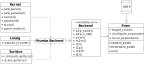
\includegraphics {figures/software.pdf}}
    \caption{Simplified UML model of all PyExaFMM components. Trees and operators are precomputed and stored in the HDF5 database. The `Fmm' object which acts as the user interface, all other components are modules consisting of methods on operating on arrays.}
    \label{fig:design}
\end{figure*}

\section{DIFFERENCES WITH EXAFMM-T}

- PyExaFMM's tree data structure influence by Numba preference for linear data structure.

- A short note on the decision for M2l via SVD for FMM experts.


\section{BENCHMARKS}

- contrast multithreading impact for each kernel

- boxing cost for each kernel

- compare and contrast pyexafmm vs exafmm for a given accuracy, try and find optimum compression parameter.(?)

\section{CONCLUSION}

In this paper we've shown how to use Numba to create a performant application for an algorithm with a complex data structure. We've shown how Numba can constrain software design, and that developers must be careful in designing methods and data structures in order to experience a performance benefit. Furthermore, performance debugging for more complex applications may require more knowledge than non-software specialists can be expected to have. Therefore, despite being trivial to drop-in to an existing application, Numba can be seen to have its own learning curve for achieving performance. Despite this, we conclude that Numba is a remarkable tool. With a great deal of functionality, allowing one to develop fast, heterogenous, cross-platform numerical applications, using only Python, and it offers a platform for experimentation and prototyping.

\section{ACKNOWLEDGMENT}

SK is sported by EPSRC Studentship 2417009.

\bibliography{pyexafmm}

\bibliographystyle{ieeetr}

\begin{IEEEbiography}{Srinath Kailasa}{\,}is a PhD student in Mathematics at University College London. Contact him at srinath.kailasa.18@ucl.ac.uk.
\end{IEEEbiography}

\begin{IEEEbiography}{Tingyu Wang}{\,}is a PhD student in Mechanical Engineering at the George Washington University. Contact him at twang66@email.gwu.edu.
\end{IEEEbiography}

\begin{IEEEbiography}{Lorena. A. Barba}{\,}is a Professor of Mechanical and Aerospace Engineering at the George Washington University.  Contact her at labarba@email.gwu.edu.
\end{IEEEbiography}

\begin{IEEEbiography}{Timo Betcke}{\,}is Professor of Computational Mathematics at University College London. Contact him at t.betcke@ucl.ac.uk.
\end{IEEEbiography}

\end{document}

